\documentclass{beamer}
\usepackage{HECbeamer}
\usepackage{icomma}
\usepackage{numprint}
\title[\color{white}{MATH 60604 \S~5e - Modèle autorégressif d'ordre 1}]{\texorpdfstring{MATH 60604 \\Modélisation statistique \\ \S~5e - Modèle autorégressif d'ordre 1}{MATH 60604 \\Modélisation statistique \\ \S~5e - Modèle autorégressif d'ordre 1}}
\author{}
\institute{HEC Montréal\\
Département de sciences de la décision}
\date{} 

\begin{document}
\frame{\titlepage}

\begin{frame}
\frametitle{Choix de la structure de covariance}
\bi
\item Nous avons vu que modéliser la corrélation entre les
mesures répétées d'une même personne en supposant l'équicorrélation semblait raisonnable. 
\item Cette structure est en effet
plausible et, de plus, le paramètre qui mesurait cette covariance (ou
corrélation) était significativement différent de zéro. 
\item Mais comment savoir si cette structure est adéquate? Une autre pourrait être préférable.
\item Il existe plusieurs autres modèles de covariance et \SASlang{} permet d'en spécifier
un très grand nombre. Nous en présenterons quelques-uns ici; une liste
exhaustive se trouve dans le module d'aide de \SASlang{}.
\ei
\end{frame}

\begin{frame}
\frametitle{Choix de la structure de covariance}
\bi
\item Dans beaucoup de cas, la structure de covariance est considérée comme un
paramètre de nuisance. Plus précisément, souvent l'intérêt premier de l'étude
concerne les effets des variables explicatives, $\bs{\beta}$. 
\item Dans ce cas, la structure
de covariance ne nous intéresse pas en tant que tel mais nous savons qu'il est
important de la modéliser adéquatement afin que l'inférence sur $\bs{\beta}$ soit
valide. 
\item Dans ce cas, il est possible de baser le choix de la structure de
covariance sur les critères d'information si les modèles ne sont pas emboîtés, pour autant qu'ils aient les mêmes variables explicatives (si ajusté avec la méthode REML).
\ei
\end{frame}

\begin{frame}
\frametitle{Structure auto-régressive}
\bi
\item La structure équicorrélation utilisée plus tôt suppose que la corrélation
entre deux observations est toujours la même. 
\item Lorsque nous avons à faire à
des mesures répétées prises à différents moments dans le temps, comme ici, 
il est possible que la corrélation entre deux observations dépende du temps
écoulé entre les mesures. 
\item C'est-à-dire, on pourrait croire que plus les
observations sont rapprochées dans le temps, plus elles sont corrélées. La
structure \alert{$\mathsf{AR}(1)$} (\alert{autorégressive d'ordre 1}) est une structure simple qui permet
de saisir en partie cet aspect. 
\item Tout comme la structure équicorrélation, la
structure $\mathsf{AR}(1)$ comporte deux paramètres: un paramètre de corrélation $\rho$ et
un paramètre de variance $\sigma^2$.
\ei
\end{frame}

\begin{frame}
\frametitle{Structure autorégressive}
\bi
\item Pour l'individu $i$ avec cinq réponses, la matrice de corrélation est
\[
\mathbf{R}_i=
  \begin{pmatrix}
   1 & \rho & \rho^2 & \rho^3 & \rho^4\\
    \rho & 1 & \rho & \rho^2 & \rho^3\\
    \rho^2 & \rho & 1 & \rho &  \rho^2\\
       \rho^3 & \rho^2 & \rho & 1 & \rho\\
       \rho^4 & \rho^3 & \rho^2 & \rho & 1
  \end{pmatrix}.
\]
\item La matrice de covariance est
\begin{align*}
\bs{\Sigma}_i=\sigma^2  \mathbf{R}_i.
\end{align*}
\ei
\end{frame}

\begin{frame}
\frametitle{Corrélation du modèle autorégressif d'ordre un}
\bi
\item La corrélation (conditionnelle) entre deux observations
espacées par une seule période de temps (deux semaines ici) est $\rho \in (-1, 1)$. 
\item La corrélation entre deux observations espacées par deux périodes de temps (quatre
semaines) est $\rho^2$, et ainsi de suite. 
\item Lorsque $0 <\rho<1$, la suite $\rho, \rho^2, \rho^3, \rho^4$, \ldots, 
est décroissante. Par conséquent, la corrélation entre deux observations
décroît exponentiellement en fonction de la différence de temps entre les deux
mesures.
\ei
\end{frame}


\begin{frame}[fragile]
\frametitle{Code \SASlang{} pour ajuster un modèle $\mathsf{AR}(1)$}
\begin{tcolorbox}[colback=white, colframe=hecblue, title=Code \SASlang{} pour ajuster un modèle $\mathsf{AR}(1)$]
\begin{verbatim}
proc mixed data=vengeance method=reml;
class id tcat;
model vengeance = sexe age vc wom t / solution;
repeated tcat / subject=id type=ar(1) r=1 rcorr=1;
run;
\end{verbatim}
\end{tcolorbox}
\end{frame}

\begin{frame}[fragile]
\frametitle{Matrice de corrélation et de covariance pour le sujet 1 du modèle $\mathsf{AR}(1)$}
\begin{center}
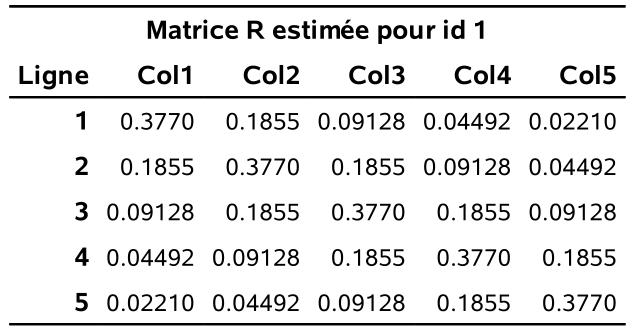
\includegraphics[width = 0.45\linewidth]{img/c5/diapos6-e15a}
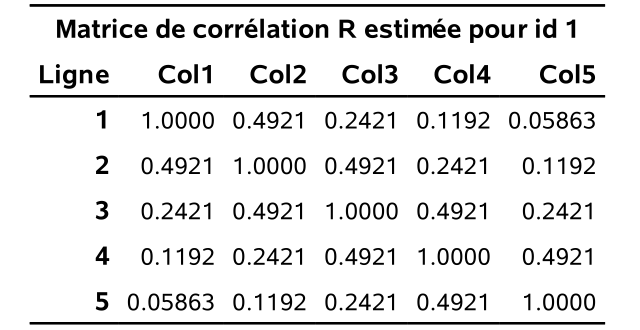
\includegraphics[width = 0.45\linewidth]{img/c5/diapos6-e15b}
\end{center}
\bi
\item On voit que la corrélation entre deux observations diminue avec le temps écoulé entre elles. 
\item C'est bien ce que nous voulions faire en choisissant la structure de covariance $\mathsf{AR}(1)$.
\ei
\end{frame}

\begin{frame}[fragile]
\frametitle{Paramètres de la structure de covariance/corrélation du modèle $\mathsf{AR}(1)$}
\begin{center}
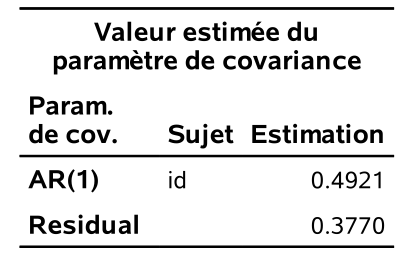
\includegraphics[width = 0.4\linewidth]{img/c5/diapos6-e16}
\end{center}
\bi
\item On voit que l'estimation
du paramètre $\rho$ est $\hat{\rho}= \numprint{0.492}$. 
\item On peut vérifier dans la matrice de corrélation du sujet $1$ que la corrélation entre $t_1$ et $t_2$ est de $ \numprint{0.492}$, que la corrélation entre $t_1$ et $t_3$ est de $ \numprint{0.492}^2= \numprint{0.24}$, etc.
\item Remarque:  dans le modèle d'équicorrélation, la corrélation entre deux
observations quelconques d'une même personne (peu importe le temps
écoulé entre les mesures) était estimée à $ \numprint{0.356}$. 

\ei
\end{frame}


\begin{frame}[fragile]
\frametitle{Estimés des paramètres de la moyenne}
\begin{center}
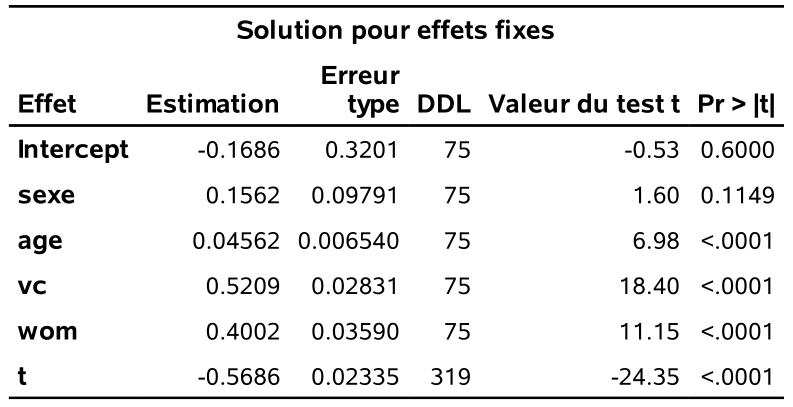
\includegraphics[width = 0.7\linewidth]{img/c5/diapos6-e17}
\end{center}
\bi
\item Les estimés des paramètres $\bs{\beta}$ sont très similaires à ceux du modèle d'équicorrélation, mais pas identiques. 
\item L'effet de toutes les variables explicatives est significatif, hormis celui du \code{sexe}. Les conclusions sont les mêmes que précédemment.
\ei
\end{frame}

\end{document}
